\documentclass[10pt]{article}

% ---------- packages ----------
\usepackage[utf8]{inputenc}
\usepackage{microtype}    % crisper spacing / margin kerning
\usepackage[margin=0.5in]{geometry}
\usepackage{xcolor}
\usepackage{booktabs}
\usepackage{multicol}
\usepackage{enumitem}
\usepackage{amsmath}
\usepackage{tikz}
\usepackage{listings}
\usepackage{titlesec}
\usetikzlibrary{positioning,shapes.geometric,arrows.meta,fit,backgrounds}

% ---------- colours ----------
\definecolor{accent}{HTML}{1A4D7A}
\definecolor{accent2}{HTML}{2E7D6B}
\definecolor{ink}{HTML}{222222}
\definecolor{muted}{HTML}{555555}
\definecolor{band}{HTML}{EEF2F6}
\definecolor{engine}{HTML}{EAF1F7}
\definecolor{proj}{HTML}{EAF3EF}
\definecolor{codebg}{HTML}{F5F7F9}

% ---------- spacing / type ----------
\setlength{\parindent}{0pt}
\setlength{\parskip}{2pt}
\setlength{\columnsep}{16pt}
\pagestyle{empty}

\titleformat{\section}{\color{accent}\bfseries\small}{\thesection}{0.5em}{}
\titlespacing{\section}{0pt}{4pt}{2pt}

% ---------- code style ----------
\lstdefinestyle{cfg}{
  basicstyle=\ttfamily\scriptsize\color{ink},
  backgroundcolor=\color{codebg},
  breaklines=true, frame=none, xleftmargin=4pt, xrightmargin=2pt,
  aboveskip=3pt, belowskip=2pt,
  keywordstyle=\color{accent}, commentstyle=\color{accent2}\itshape,
}

\newcommand{\fld}[1]{{\ttfamily\footnotesize #1}}

\begin{document}

% ===================== HEADER =====================
{\color{accent}\LARGE\bfseries Multi-Source Candidate Data Transformer}\\[2pt]
{\color{muted}\footnotesize Stage 1 \textemdash{} Technical Design \quad$\bullet$\quad
\textbf{Harsh} \quad$\bullet$\quad harshsahuhh@gmail.com}

\vspace{3pt}
\colorbox{band}{\parbox{\dimexpr\textwidth-2\fboxsep}{\footnotesize
\textbf{North star:} the system optimises for one thing \textemdash{}
\emph{never be confidently wrong}. ``Wrong-but-confident is worse than
honestly-empty.'' Every design choice below is derived from that principle plus
the brief's four constraints: \textbf{deterministic, explainable, robust, scalable}.
}}

\vspace{4pt}

% ===================== ARCHITECTURE DIAGRAM =====================
{\color{accent}\small\bfseries Architecture \textemdash{} truth is built once, then projected}

\vspace{2pt}
\begin{center}
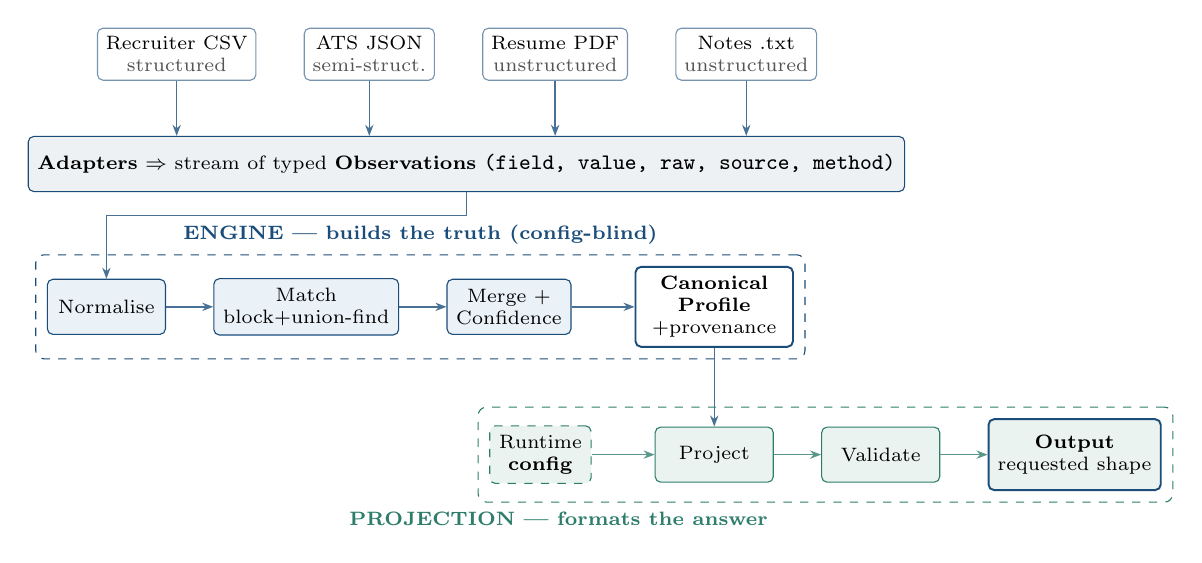
\begin{tikzpicture}[
  font=\scriptsize,
  node distance=5mm and 6mm,
  src/.style={draw=accent!60, fill=white, rounded corners=2pt, minimum height=6mm, inner sep=3pt, align=center},
  stage/.style={draw=accent, fill=engine, rounded corners=2pt, minimum height=7mm, minimum width=15mm, align=center},
  pstage/.style={draw=accent2, fill=proj, rounded corners=2pt, minimum height=7mm, minimum width=15mm, align=center},
  store/.style={draw=accent, line width=0.7pt, fill=white, rounded corners=2pt, minimum height=9mm, minimum width=20mm, align=center},
  cfg/.style={draw=accent2, dashed, fill=proj, rounded corners=2pt, minimum height=7mm, align=center},
  arr/.style={-{Stealth[length=4pt]}, accent!80, line width=0.5pt},
]

% sources
\node[src] (csv)   {Recruiter CSV\\{\color{muted}structured}};
\node[src, right=of csv] (ats) {ATS JSON\\{\color{muted}semi-struct.}};
\node[src, right=of ats] (res) {Resume PDF\\{\color{muted}unstructured}};
\node[src, right=of res] (note){Notes .txt\\{\color{muted}unstructured}};

% adapters -> observations
\node[stage, below=7mm of ats.south east, xshift=4mm, minimum width=92mm, fill=accent!8] (obs)
  {\textbf{Adapters} $\Rightarrow$ stream of typed \textbf{Observations} \fld{(field, value, raw, source, method)}};

\draw[arr] (csv.south)  -- (obs.north -| csv.south);
\draw[arr] (ats.south)  -- (obs.north -| ats.south);
\draw[arr] (res.south)  -- (obs.north -| res.south);
\draw[arr] (note.south) -- (obs.north -| note.south);

% engine pipeline row
\node[stage, below=11mm of obs.south west, xshift=10mm] (norm) {Normalise};
\node[stage, right=of norm] (match) {Match\\{\scriptsize block+union-find}};
\node[stage, right=of match] (merge) {Merge +\\Confidence};
\node[store, right=8mm of merge] (canon) {\textbf{Canonical}\\\textbf{Profile}\\{\scriptsize +provenance}};

\draw[arr] (obs.south) -- ++(0,-3mm) -| (norm.north);
\draw[arr] (norm) -- (match);
\draw[arr] (match) -- (merge);
\draw[arr] (merge) -- (canon);

% projection side
\node[pstage, below=10mm of canon, align=center] (proj) {Project};
\node[pstage, right=of proj] (val) {Validate};
\node[store, right=of val, fill=proj] (out) {\textbf{Output}\\{\scriptsize requested shape}};
\node[cfg, left=8mm of proj] (config) {Runtime\\\textbf{config}};

\draw[arr] (canon.south) -- (proj.north);
\draw[arr, accent2!80] (config.east) -- (proj.west);
\draw[arr, accent2!80] (proj) -- (val);
\draw[arr, accent2!80] (val) -- (out);

% boundary boxes
\begin{scope}[on background layer]
  \node[draw=accent, dashed, rounded corners=3pt, inner sep=4pt, fit=(norm)(match)(merge)(canon), label={[accent,font=\scriptsize\bfseries]above:ENGINE \textemdash{} builds the truth (config-blind)}] {};
  \node[draw=accent2, dashed, rounded corners=3pt, inner sep=4pt, fit=(config)(proj)(val)(out), label={[accent2,font=\scriptsize\bfseries]below left:PROJECTION \textemdash{} formats the answer}] {};
\end{scope}

\end{tikzpicture}
\end{center}

\vspace{1pt}

% ===================== TWO COLUMN BODY =====================
\begin{multicols}{2}
\footnotesize

\section{Pipeline}
\fld{detect\,$\to$\,extract\,$\to$\,normalise\,$\to$\,match\,$\to$\,merge\,$\to$\,project\,$\to$\,validate.}
Each adapter turns one raw source into observations; nothing downstream sees a
raw source again, so \textbf{adding a source = one adapter, zero changes
elsewhere}. The engine builds one fixed internal record; projection is the only
config-aware code. \emph{Why:} this boundary is what keeps output changes from
ever touching resolution logic.

\section{Canonical schema \& normalised formats}
\vspace{-2pt}
{\renewcommand{\arraystretch}{1.05}\setlength{\tabcolsep}{3pt}
\begin{tabular}{@{}p{2.05cm}p{4.0cm}@{}}
\toprule
\textbf{Field} & \textbf{Normalised form} \\
\midrule
phones & E.164 (\fld{+14155550182}) \\
location & ISO-3166 alpha-2 country \\
links & object \fld{\{linkedin, github, portfolio, other[]\}} \\
experience & dates $\to$ \fld{YYYY-MM} (+\,\fld{present}), +\,summary \\
education & \fld{\{institution, degree, field, end\_year\}} \\
skills & canonical names (\fld{JS}$\to$JavaScript) \\
emails & lower-cased, deduped, typo-suppressed \\
\bottomrule
\end{tabular}}

A normaliser that cannot parse a value returns \fld{null}; the value is dropped,
never invented.

\section{Match, merge \& confidence}
\textbf{Match keys} (priority): email\,$\to$\,phone\,$\to$\,name+company; matches
clustered by \emph{blocking + union-find} so cost stays near-linear at thousands
of records. \textbf{Each observation has}
\[ s \;=\; \text{trust}_{\text{source}} \times \text{reliability}_{\text{method}} \]
The strongest camp wins a single-valued field; multi-valued fields union+dedupe.
\textbf{Confidence} is a noisy-OR over agreeing evidence
\[ c \;=\; 1 - \textstyle\prod_i (1 - s_i) \]
so corroboration \emph{raises} confidence (an average wouldn't) and conflict
\emph{discounts} the winner. Below a floor, a single value is emitted \fld{null}.
Trust weights live in a config table (policy), separate from merge logic
(mechanism).

\columnbreak

\section{Configurable output (the twist)}
Projection selects a subset, remaps via a \fld{from}-path language
(\fld{emails[0]}, \fld{links.github}, \fld{skills[].name}), toggles
confidence/provenance, and applies a per-field policy
\fld{null\,|\,omit\,|\,error}, then validates against the
\emph{requested} schema.

\begin{lstlisting}[style=cfg]
{ "fields": [
  {"path":"full_name","required":true},
  {"path":"primary_email","from":"emails[0]"},
  {"path":"phone","from":"phones[0]","normalize":"E164"},
  {"path":"github","from":"links.github"},
  {"path":"portfolio","from":"links.portfolio","on_missing":"omit"}
], "include_confidence": true }
\end{lstlisting}
\vspace{-2pt}
$\Rightarrow$ \fld{\{"full\_name":"Maya R. Chen",}\\
\fld{\phantom{$\Rightarrow$ }"primary\_email":"maya.chen@example.com",}\\
\fld{\phantom{$\Rightarrow$ }"phone":"+14155550182",}\\
\fld{\phantom{$\Rightarrow$ }"github":"github.com/mayachen"\}}\\
({\footnotesize\fld{portfolio} omitted \textemdash{} no source had it}).

\section{Edge cases}
\vspace{-2pt}
{\renewcommand{\arraystretch}{1.05}\setlength{\tabcolsep}{3pt}
\begin{tabular}{@{}p{1.95cm}p{4.1cm}@{}}
\toprule
\textbf{Case} & \textbf{Handling} \\
\midrule
phone in 3 formats & all $\to$ one E.164; corroborated \\
typo'd email & near-dup of verified $\to$ suppressed \\
title conflict & higher-trust source wins; logged \\
\fld{Java} vs \fld{JavaScript} & fuzzy match refused below 88\% \\
corrupt source & yields 0 obs, logs, run continues \\
field nobody has & stays \fld{null}; never invented \\
\bottomrule
\end{tabular}}

\section{Rejected alternatives \& descoping}
\textbf{LLM/ML resolution} \textemdash{} rejected: non-deterministic and
untraceable, and would confidently mis-map \fld{Java}$\to$\fld{JavaScript} (the
exact failure we must avoid). \textbf{Last-write-wins merge} \textemdash{}
rejected: can't explain or score. \textbf{Deliberately out of scope under time:}
a UI (CLI suffices per brief), a datastore, and ML entity-resolution \textemdash{}
blocking + strong keys is the right complexity here.

\end{multicols}

\end{document}
